\documentclass{article}
\usepackage[utf8]{inputenc}
\usepackage{geometry}
\usepackage{longtable}
\usepackage{graphicx} % For including images
\usepackage{hyperref} % For hyperlinks

\geometry{
 a4paper,
 total={170mm,257mm},
 left=20mm,
 top=20mm,
}

\title{Software Architecture of Train Inter Payment System (TrIP)}
\author{Group 04}
\date{\today}

\begin{document}

\maketitle
\newpage

\section*{Product Introduction}
The Train Inter Payment System (TrIP) is a collaborative project initiated by three railroad tycoons to streamline the payment process for train travel. These tycoons, operating a network connecting towns, industries, and a university, aim to address the interoperability issues of their existing payment systems. TrIP will feature smart payment terminals at each station, enabling direct communication for subscription validation or single-fare payments. This system, underpinned by a service-based architecture, involves critical components like payment terminals and tycoon-specific systems. It's designed with key stakeholder requirements in mind: maintainability and operational efficiency for the owner, usability and reliability for the tycoons, and usability and security for passengers. The project seeks to ensure passengers can easily manage payments and subscriptions across the network, enhancing the overall travel experience while safeguarding user data.

\newpage
\subsection{Decision 3: Routes management}

\subsection*{Status}
Accepted.

\subsection*{Architectural Summary}
% TODO

\subsection*{Concern}
The concern is to facilitate a seamless travel planning experience for passengers by ensuring the system can accurately and efficiently gather available route options from various tycoon systems and present them based on the user's criteria of price, time, and subscription status.

\subsection*{Context}
In the context of enhancing the TrIP system's ability to provide optimized travel options, we face the challenge of efficiently querying multiple tycoon systems to gather route information that aligns with passenger preferences and existing subscriptions.
The decision is centered on the system's interface with tycoon systems to retrieve and optimize route data, which impacts the functionality and performance of the terminal's route planning features for the passengers.

\subsection*{Criteria}
The key criteria for the decision include:
\begin{itemize}
    \item User-friendly passenger interface.
    \item Comprehensive and diverse route options.
    \item Accurate representation of options based on multiple factors.
    \item Streamlined integration with multiple tycoon systems.
\end{itemize}

\subsection*{Option 1: Direct Tycoon Integration}
Terminals directly interface with each tycoon system and the central database to collate route options. The route optimizer processes this data to present optimal travel solutions. This requires our system to have APIs to query each of the tycoons systems.
\begin{figure}[ht]
    \centering
    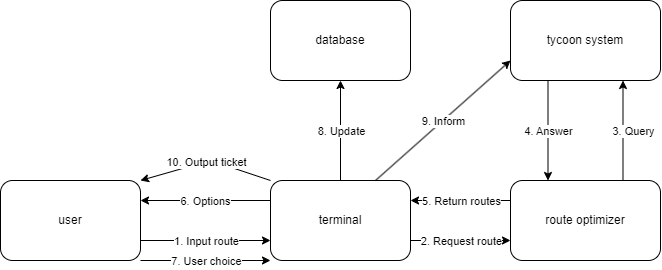
\includegraphics[width=\textwidth]{drawings/decision3_drawings/direct.png}
    \caption{Direct Data Management Interface}
    \label{fig:direct-data-interface}
\end{figure}

\subsection*{Option 2: Centralized Route Management Module}
A central route data management module acts as an intermediary between terminals and tycoon systems, standardizing and aggregating data before it is processed by the route optimizer. A database containing the timetables will be kept up to date by the tycoon (possibly though an API, this will be the focus of a later decision). The route data management system might cache optimized routes, in order to minimize database requests. A module specialized in running optimizations with the data it is provided with interacts solely with the Route Management Module.
\begin{figure}[ht]
    \centering
    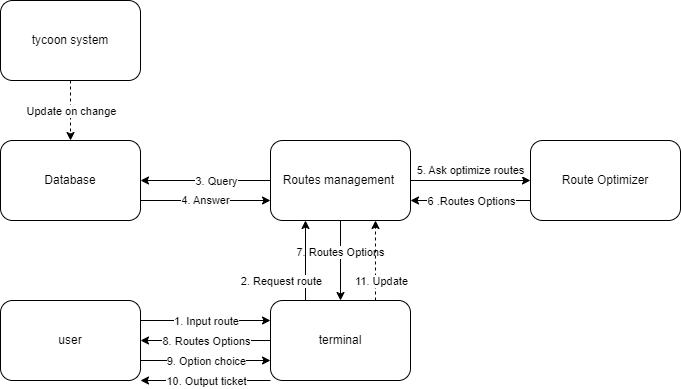
\includegraphics[width=\textwidth]{drawings/decision3_drawings/centralized.png}
    \caption{Centralized Route Management Module. Dashed lines represents steps to be explained in future decisions.}
    \label{fig:centralized-data-interface}
\end{figure}
  
\subsection*{Decision}
We have decided to proceed with Option 2: Centralized Route Management Module. This decision is based on the module's ability to simplify the data flow between systems and to effectively manage the complexity of integrating with multiple tycoon systems. The introduction of a separate data management module will allow for greater flexibility and scalability.

\subsection*{Consequences}
\textbf{Positive Consequences:}
\begin{itemize}
    \item Simplified data flow between the trip system and tycoons.
    \item Improved scalability and maintainability of the system.
    \item Easier to integrate with current and future tycoon systems.
\end{itemize}
\textbf{Negative Consequences:}
\begin{itemize}
    \item Initial development and integration effort for the new module.
    \item Potential complexity in data synchronization between modules.
\end{itemize}
This approach is expected to provide a solid foundation for the system's scalability and adaptability to evolving requirements and stakeholder needs.
\newpage

\section*{Decision 4: How to integrate subscription to route optimization module}

\subsection*{Status}
Review

\subsection*{Architectural Summary}
In developing the TrIP system, we explore subscription model architectures that align railway tycoons' need for flexibility with passengers' demand for simplicity. 
We assess the trade-offs between unified and tycoon-specific models to enhance both operational autonomy and passenger convenience.

\subsection*{Concern}
A user wants to know the available tickets from A-B. 
Connected user stories: 16 (passenger want one payment for many trains), 23 (tycoon wants easy integration with their system)

\subsection*{Context}
When passengers want to go from station A to station B, they want to be able to use all the subscription they have and pay for the trains belonging to tycoons they are not subsribed to.
The terminal has to communicate with the tycoon systems to verify subscriptions and check routes.

\subsection*{Criteria}
\begin{itemize}
\item Ease of use for the passenger.
\item Multiple route options for the user.
\item The system returns to user usable options based on price/time/availability/subscription.
\item Simple integration with the tycoon systems.
\end{itemize}

\subsection*{Option 1: Introduction of a subscription manager tool, route optimizer needs to take subs into consideration.}
We want to include a Subscription Manager module to our functional view. 
Such a module has the responsibility to verify subscriptions, communicating with the tycoon system.
Furthermore, the Route Optimizer module needs to be able to optimize wrt price given that the passenger holds some subscription.
The idea is to add an optional initial iteration to the sequence of actions sketched in decision3.
This requires a way to communicate the subscription to the terminal, be it a QR code, a code or a magnetic card. 
This should be the topic of another decision.

The functional view schema is in my bag.

\subsection*{Option 2}

\subsection*{Decision}

\subsection*{Consequences}
\textbf{Positive Consequences:}
\begin{itemize}
\end{itemize}
\textbf{Negative Consequences:}
\begin{itemize}
\end{itemize}
\newpage
\section*{Decision 5: How to handle quickly filling trains?}

\subsection*{Status}
Review

\subsection*{Architectural Summary}
QA scenario (availability): When a route is requested by a passenger to a terminal, the terminal verifies that the trains arent fully booked and then proceeds to
ask for the payment.
It could happen that at the same time another passenger buys the last ticket. This is relevant expecially in peak hours, which are typically important for commuters and students.

\subsection*{Concern}
Passenger wants minimum usability and availability. Also, we (and the tycoons) don't want to have customer service issues.
Connected user stories: 15 (passenger don't want to pay for unavailable routes)

\subsection*{Context}


\subsection*{Criteria}
\begin{itemize}
\item Not too many requests to tycoon systems.
\item Performance, to avoid passenger have a bad user experience.
\item Don't allow to pay two users for the same spot.
\end{itemize}

\subsection*{Option 1: }
We should maintain a database where info about scheduled trains is stored. 
This database should be updated by the terminal when a ticket has been bought.
This database should ask periodically to the tycoon systems updates on schedules.
When the user select that they want to pay for a specific ticket, that ticket should be locked, so that no one else can buy it. 
If the payment is not ultimated, it can be unlocked.

\subsection*{Option 2: }

\subsection*{Decision}

\subsection*{Consequences}
\textbf{Positive Consequences:}
\begin{itemize}
\end{itemize}
\textbf{Negative Consequences:}
\begin{itemize}
\end{itemize}
\newpage
\section*{Decision 6: How to handle train disruptions?}

\subsection*{Status}

\subsection*{Architectural Summary}


\subsection*{Concern}


\subsection*{Context}


\subsection*{Criteria}
\begin{itemize}
\end{itemize}

\subsection*{Option 1: }

\subsection*{Option 2: }

\subsection*{Decision}

\subsection*{Consequences}
\textbf{Positive Consequences:}
\begin{itemize}
\end{itemize}
\textbf{Negative Consequences:}
\begin{itemize}
\end{itemize}
\newpage
\section*{Decision 7: How and what to communicate to customer service?}

\subsection*{Status}

\subsection*{Architectural Summary}


\subsection*{Concern}


\subsection*{Context}


\subsection*{Criteria}
\begin{itemize}
\end{itemize}

\subsection*{Option 1: }

\subsection*{Option 2: }

\subsection*{Decision}

\subsection*{Consequences}
\textbf{Positive Consequences:}
\begin{itemize}
\end{itemize}
\textbf{Negative Consequences:}
\begin{itemize}
\end{itemize}
\newpage


% \begin{table}[H]
    \resizebox{\textwidth}{!}{%
    \begin{tabular}{|l|c|c|c|c|c|c|c|c|c|c|c|}
    \hline
    \textbf{User Story} & \textbf{Usability} & \textbf{Performance} & \textbf{Security} & \textbf{Modifiability} & \textbf{Deployability} & \textbf{Energy Efficiency} & \textbf{Availability} & \textbf{Safety} & \textbf{Integrability} & \textbf{Testability} & \textbf{Accessibility} \\
    \hline
    1. Frequent traveler monthly pass & + &  &  &  &  &  &  &  &  &  &  \\
    \hline
    2. Check travel card balance & + &  &  &  &  &  &  &  &  &  &  \\
    \hline
    3. Subscription notifications & + &  &  &  &  &  &  &  &  &  &  \\
    \hline
    4. Mobile app management & + &  &  &  & - &  &  &  &  &  &  \\
    \hline
    5. Carbon footprint tracking &  & - &  &  &  & + &  &  &  &  &  \\
    \hline
    6. Accessible services info & + &  &  &  &  &  &  & + &  &  &  \\
    \hline
    7. Voice-activated features & + &  &  & - & - &  &  &  &  &  & + \\
    \hline
    8. Simple interface for elders & + &  &  & + &  &  &  &  &  &  &  \\
    \hline
    9. Multilanguage options & + &  &  & - &  &  &  &  &  &  &  \\
    \hline
    10. Quick access to popular trips & + & - &  & - &  &  &  &  &  &  &  \\
    \hline
    11. Scan student card for benefits & + &  &  & - &  &  &  &  &  &  &  \\
    \hline
    12. Single transaction for subscriptions & + & - &  &  &  &  &  &  &  &  &  \\
    \hline
    13. Charge train cards at terminal & + &  &  & - &  &  &  &  &  &  &  \\
    \hline
    14. Interface for visually impaired & + &  &  &  &  &  &  &  &  &  & + \\
    \hline
    15. Block payment for blocked routes & + & - &  & - &  &  &  &  &  &  &  \\
    \hline
    16. Single ticket across all networks & + & - &  & - &  &  &  &  &  &  &  \\
    \hline
    17. Subscriptions advice for commuting & + & - &  & - &  &  &  &  &  &  &  \\
    \hline
    18. Adherence to security standards &  &  & + & - &  &  &  &  & - & - &  \\
    \hline
    19. Detailed reporting for government & + &  &  & - &  &  &  &  & - &  &  \\
    \hline
    20. Reduced fares for eligible populations & + & - &  & - &  &  &  &  &  &  &  \\
    \hline
    21. Revenue tracking for tycoons & + & - &  & - &  &  &  &  &  &  &  \\
    \hline
    22. Exclusive promotions & + &  &  & - &  &  &  &  &  &  &  \\
    \hline
    23. Payment system integration & + &  &  & - &  &  &  &  & + & - &  \\
    \hline
    24. Access to analytics &  &  &  & - &  &  &  &  & + &  &  \\
    \hline
    25. Assistance for ticket purchases & + &  &  & - &  &  &  &  &  &  &  \\
    \hline
    26. Temporary fare adjustments &  &  &  & - &  & + &  &  &  &  &  \\
    \hline
    27. Integration with maintenance tools &  &  &  & - &  & + &  &  &  &  &  \\
    \hline
    28. Audit trails and compliance &  &  &  & - &  &  &  &  &  &  &  \\
    \hline
    \end{tabular}%
    }
    \caption{User Stories and Quality Attributes}
\end{table}

\section*{Context Viewpoint}
\subsection*{View: \textless{}Name\textgreater{}}
\subsubsection*{Model}
Place here the model representation of the view

\subsubsection*{Description}
Short description of the view

\subsubsection*{Glossary of Elements}
\begin{longtable}{lll}
Id & Name & Description \\
\end{longtable}

\subsection*{Analysis on Perspectives}
Describe how the view satisfies the different perspectives. 

\section*{Functional Viewpoint}

\section*{Information Viewpoint}

\section*{Concurrency Viewpoint}

\section*{Development Viewpoint}

\section*{Deployment Viewpoint}

\end{document}
